\chapter{On-Chip Diagnosis Architecture}
\label{chap:diag}

This chapter describes and evaluates a diagnosis architecture developed for performing on-chip diagnosis.
%
While each core/uncore in the System on Chip (SoC) design has a different test set and TRAX fault dictionary, the on-chip diagnosis architecture is used for all diagnosis activities.
%
The CASP test controller~\cite{li08} periodically selects a core/uncore for testing, isolates it from the rest of the SoC (saving critical state and re-routing computational tasks), applies a high-quality test set to the core/uncore while recording the test responses, and finally re-integrates the tested core/uncore within the system (restoring saved state and restoring tasks back to the tested core/uncore).
%
If any failures are detected, the on-chip diagnosis architecture is used to diagnose the failing test responses to localize the failure within the core/uncore.
%
More details on the system test and diagnosis architecture are provided in Section~\ref{sec:diag_system_test_and_diag}.
%
The high-quality test sets needed to detect the targeted early-life and wear-out failures require the use of off-chip storage, which is also used to store the fault dictionary data (details in Section~\ref{sec:diag_off_chip_hw}).
%
The TRAX diagnosis architecture, an on-chip hardware implementation of hierarchical fault diagnosis, is described in Section~\ref{sec:diag_on_chip_hw}.
%
Experiments in Section~\ref{sec:diag_exp} evaluate the on-chip diagnosis architecture.
%
Specifically, we simulate thousands of circuit failures using tests generated by a commercial tool.
%
The ``tester'' response produced by each simulation is fed to the on-chip diagnosis architecture to perform the on-chip diagnosis.
%
The result of each diagnosis is then evaluated for accuracy and resolution, that is, how many faulty modules did diagnosis report (i.e., resolution), and, among the faulty modules reported, did one contain the simulated failure (i.e., accuracy).

\section{System Test and Diagnosis}
\label{sec:diag_system_test_and_diag}

The on-chip test process adopted here leverages CASP (Concurrent Autonomous chip self-test using Stored test Patterns)~\cite{li08}.
%
In CASP, a small amount of additional hardware enables the re-use of DFT logic to test the chip post-manufacturing.
%
High-quality test and diagnosis data are stored in off-chip memory and loaded into the chip as needed during test and diagnosis of a particular core/uncore.
%
Each unique core/uncore in a system requires a set of test and diagnosis data.
%
Off-chip data for each core/uncore is organized as a series of tests, and the data for each test includes (i) a pair of test vector inputs (called $V_1$ and $V_2$), (ii) the expected test response, (iii) a bitmask indicating which response bits should be checked against the expected test response, and (iv) the corresponding column of the fault dictionary.

CASP consists of four phases.
%
First, the CASP controller identifies the next component to test, such as a processing core or an uncore component (e.g., memory controller).
%
Next, the selected core/uncore is then isolated from the rest of the system, saving critical state and re-routing computational tasks.
%
Third, the actual tests are applied one at a time by (i) loading the relevant test data from off-chip into the on-chip buffer, (ii) test application via the DFT logic, and (iii) core/uncore response evaluation for incorrect behavior that results in a one-bit pass/fail status for each test.
%
Finally, once all tests have been applied, the CASP controller reintegrates the core/uncore with the rest of the system and resumes its execution.

The objective of on-chip diagnosis is to determine which module of the core/uncore is most likely the reason for any observed test failure.
%
For on-chip diagnosis, the previously-described TRAX fault dictionary is used, which stores a single bit for fault/test pairs to indicate if the fault is detected by the corresponding test pair.
%
Using the TRAX fault dictionary in conjunction with the pass/fail test response from the CASP test execution, a list of potentially responsible modules is generated.
%
Specifically, starting with a list of all faults within the tested core/uncore dictionary, each failing test response is used one at a time to eliminate any faults that are not detected by the corresponding test.
%
When all test responses have been processed, what remains is a list of TRAX faults consistent with the observed behavior.
%
Each fault in this list belongs to one of the modules of the tested core/uncore.
%
Moreover, counting the number of potentially responsible faults in each module gives an indication of the likelihood of finding the actual defect in each of the implicated modules, and thus is reported as the outcome of on-chip diagnosis.

On-chip diagnosis can be performed in two different situations, the first being failure prediction, where an accelerated clock is used to detect pending failures.
%
In this situation, the diagnosis can be run in the background with no performance overhead and only a little extra power consumption.
%
The other situation is after a real failure is detected, implying that the core/uncore is unable to be used because it has failed.
%
For this case, the time required for diagnosis is indeed important because there is performance overhead associated with diagnosing the failure and deploying fault repair, replacement, or avoidance before execution can resume.


\section{Off-Chip Hardware}
\label{sec:diag_off_chip_hw}

To enable on-chip test and diagnosis requires the addition of specialized hardware, both off and on the chip itself.
%
The off-chip hardware includes memory for storing the test and dictionary data, such as non-volatile flash memory, system DRAM, or on disk.
%
The use of off-chip data storage is reasonable given the trend towards availability of high-density, low-cost flash memory for off-chip storage~\cite{li08}.
%
Additionally, the high-quality test patterns required for ELF and wear-out failure detection cannot easily be produced using conventional BIST techniques.
%
While there are special techniques to achieve high test coverage with BIST~\cite{touba96,wunderlich96}, these techniques can be expensive to implement.
%
Finally, the use of off-chip storage allows the test and dictionary data to be updated (patched), if better-performing data is later identified.
%
Patching might become necessary to deal with a new strain of failure that may occur later in the life cycle of the system, for example, or to incorporate failure knowledge gained from physical failure analysis (PFA) after manufacturing.

%\vskip 0.5em%
\begin{figure}[hbtp]
\centering

\includegraphics[width=1.0\columnwidth]{fig_off_chip_memory}
\caption{For each unique core/uncore, separate fault dictionaries are constructed and stored in off-chip memory along with the required test data.}
\label{fig:diag_off_chip_memory}
\end{figure}
%\vskip 0.5em%

Each unique core (e.g., CPU, FPU, or GPU) and uncore (DRAM controller, cache controller, etc.) has its own set of test and diagnosis data in the off-chip storage.
%
The use of multiple fault dictionaries, one per tested core/uncore, is justified since it is the smallest testable/repairable object in the chip.
%
Using separate dictionaries reduces the overall amount of dictionary data since faults from the tested core/uncore do not have to be distinguished from all the faults of all the remaining untested cores/uncores.
%
The actual data stored in the off-chip memory is illustrated in Figure~\ref{fig:diag_off_chip_memory}, and consists of an array of test and diagnosis data for each core/uncore, with one row for each test.
%
Additionally, a small amount of core/uncore-specific parameters are stored off-chip, including the fault count, test vector count, and the boundary values used by the diagnosis architecture (Section~\ref{sec:diag_on_chip_hw}) to determine which modeled faults belong to which module of the core/uncore.

The test and diagnosis data stored for each test consists of the pair of test vectors called $V_1$ and $V_2$, which are applied to the core/uncore using (mostly) existing DFT under the control of the CASP test controller~\cite{li08,li10,li13}.
%
Also stored is the expected response of the core/uncore to the applied test vector pair and a response mask indicating the validity of each response bit.
%
Finally, each test also has associated diagnosis data, specifically the corresponding test column of the core/uncore fault dictionary.
%
As previously mentioned, a fault dictionary can be thought of a table of fault responses (or some subset or function of the fault responses) with one row for each modeled fault and one column for each applied test.
%
For a TRAX hierarchical fault dictionary, each column indicates which modeled faults could cause a failure for the corresponding test.
%
A dictionary test column is used for the on-chip diagnosis; specifically, it is used to eliminate faults that could not possibly explain the observed test failures, leaving only those ``candidate'' faults that could be responsible for the faulty behavior.

Details of the size of the off-chip storage deserve further discussion.
%
The test vectors $V_1$ and $V_2$, the expected response, and the response mask all require as many bits as the length of the scan chain for the corresponding core/uncore.
%
The dictionary test column data requires one bit per fault.
%
All of this data (vectors, response, mask, and dictionary column) is repeated for each test in the core/uncore test set.
%
We calculate the required off-chip storage for one of the largest analyzed circuits, the NCU uncore from the OpenSPARC T2 processor design~\cite{sun11}.
%
With 16,582 bits in the scan chain and 21,537 faults in the dictionary, 10.73 KB of off-chip storage are required for each of the 211 tests required for NCU, bringing the total to 2.21 MB.

Because these tests are applied during the normal operation of the system, user-visible test execution time should be minimized.
%
Fortunately, the off-chip test data can be pre-fetched into on-chip buffers during normal operation (before the selected core/uncore is isolated from the system for test), hiding the access and transfer time.
%
If test results indicate that the core/uncore has failed any applied tests, dictionary data is loaded from off-chip storage and used by the diagnosis architecture.
%
When a faulty core/uncore is detected, the system must take some corrective action (repair, replace, or avoid the faulty module), so the additional time required to load the dictionary data is small compared to the recovery time.


\section{TRAX On-Chip Hardware}
\label{sec:diag_on_chip_hw}

In addition to the off-chip storage, there is dedicated on-chip hardware for actually performing diagnosis that we call the Diagnosis Architecture (DA); its structure and operation are given in Figure~\ref{fig:diag_trax_architecture} and Algorithm~\ref{alg:diag_on_chip_diag}, respectively.

\begin{algorithm}
\centering
\caption[On-Chip Diagnosis]{-- On-Chip Diagnosis}
\label{alg:diag_on_chip_diag}
\begin{algorithmic}[1]
\STATE perform test and store response in PF
\STATE reset FI counter and $M$ module counters in FMIC
\STATE initialize $(M - 1)$ module index registers (MIRs)
\FOR{$c = 0$ \TO $\lceil F / k \rceil$}
  \STATE reset fault accumulator (FA[0:$k$-1] = 0)
    \FOR{$i=0$ \TO $(T-1)$}
        \STATE FA[0:$k$-1] $|=$ ({\raise.17ex\hbox{$\scriptstyle\sim$}}fault[$ck$:($c$+1)$k$-1][$i$] \& PF[0])
        \STATE PF = PF $>>$ 1
    \ENDFOR
    \FOR{$i=0$ \TO $(k-1)$}
        \FOR{$j=0$ \TO $(M-1)$}
            \IF{FA[0] == 0}
                \IF{lower\_bound[$j$] $\leq$ FI $<$ upper\_bound[$j$]}
                    \STATE module\_count[$j$]++
                \ENDIF
            \ENDIF
        \ENDFOR
        \STATE FA = FA $>>$ 1
        \STATE FI++
    \ENDFOR
    \FOR{$i=0$ \TO $(T_{max} - T)$}
        \STATE PF = PF $>>$ 1
    \ENDFOR
\ENDFOR
\end{algorithmic}
\end{algorithm}

%\vskip 0.5em%
\begin{figure}[hbtp]
\centering
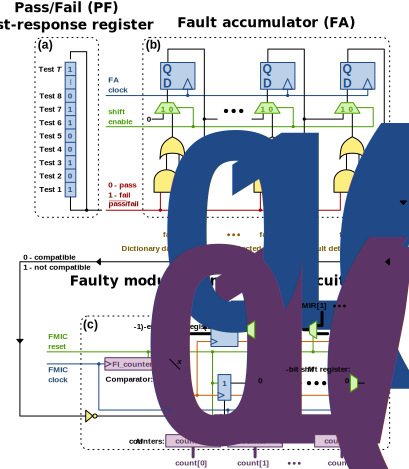
\includegraphics[width=\columnwidth]{fig_trax_architecture}
\caption{The diagnosis architecture: (a) the Pass/Fail (PF) test response register stores test responses in a circular buffer, (b) the fault accumulator (FA) tracks faults compatible with observed incorrect behavior, (c) the faulty module identification circuitry (FMIC) maps faults to core/uncore modules, tracking how many compatible faults are within each module.}
\label{fig:diag_trax_architecture}
\end{figure}
%\vskip 0.5em%

Test execution produces a pass/fail bit for each test vector pair, which is stored in an on-chip circular shift register called the PF (line 1 of Algorithm~\ref{alg:diag_on_chip_diag}, Figure~\ref{fig:diag_trax_architecture}a), where a one indicates the test has failed (Tester Fail) and a zero indicates a test has passed (Tester Pass).
%
The dictionary diagnosis data for the $F$ faults of the tested core/uncore is associated with each test and includes a pass/fail list of $F$ binary values, one per fault, where a one indicates that the corresponding fault is detected by the test (Simulation Fail), and a zero indicates a non-detection (Simulation Pass).
%
The pass/fail test response in the PF is compared with the pass/fail simulation response of each fault (line 7 of Algorithm~\ref{alg:diag_on_chip_diag}).
%
A fault is eliminated if there is any one-sided failure disagreement between the test response and the fault response stored in the dictionary.
%
Specifically, if there is a Tester-Fail Simulation-Pass (TFSP) found for any test, then the corresponding fault is eliminated from consideration.
%
Elimination of a fault using TFSP is justifiable since the TRAX fault model is very conservative in nature.
%
In other words, it is very unlikely for a slowed standard cell to fail a given test without the corresponding fault also being detected given both the generalized activation and fault effect propagation properties that characterize the TRAX fault model (as detailed in Chapter~\ref{chap:trax}, Section~\ref{sec:trax_trax}).

Figure~\ref{fig:diag_trax_architecture}b shows the part of the DA responsible for finding any cases of TFSP.
%
Because the number of faults $F$ for a tested core/uncore can be large, the DA only compares $k < F$ faults at a time, tracked by the variable $c$ in the outer loop (lines 4-24 of Algorithm~\ref{alg:diag_on_chip_diag}).
%
Specifically, for a given test-vector pair $t_i \in T$, its pass/fail response bit stored in the PF is simultaneously compared with the pass/fail simulation bits from $k$ faults (line 7 of Algorithm~\ref{alg:diag_on_chip_diag}).
%
The result of each comparison is stored in a flip-flop; a zero is stored for a given fault if there is no TFSP found, otherwise a one is stored and maintained.
%
All $T$ test pairs are examined over $T$ clock cycles (lines 6-9 of Algorithm~\ref{alg:diag_on_chip_diag}) by having PF operate as a circular shift register as shown in Figure~\ref{fig:diag_trax_architecture}a.
%
The register and the associated hardware for identifying any cases of TFSP among $k$ faults are called the fault accumulator (FA).
%
Locations within the FA that store a logic zero indicate which of the $k$ faults are potentially responsible for the core/uncore failure.

The remaining portion of the DA (Figure~\ref{fig:diag_trax_architecture}c) implements the faulty module identification circuitry (FMIC).
%
The FMIC associates the potentially-responsible faults (locations in the FA with a zero stored) with their corresponding modules within the tested core/uncore.
%
Additionally, the FMIC counts the number of potentially responsible faults associated with each module, allowing their relative ranking based on the number of faults that each contains.
%
The FMIC receives the fault data from the FA register serially through its shift function (loop on lines 10-20 in Algorithm~\ref{alg:diag_on_chip_diag}).
%
A counter called the fault index (FI) is used to track which of the $F$ faults of the tested core/uncore is being examined (in Algorithm~\ref{alg:diag_on_chip_diag} line 2 resets the FI and FMIC counters, and line 19 increments FI).
%
This implies that fault data within the dictionary are arranged by modules so that all the faults for each module are adjacent.
%
Based on this fault ordering, a comparator and a bank of counters are used to count the number of potentially responsible faults that belong to each module.
%
These per-module fault counts are used to make decisions about corrective action.
%
The most straightforward decision making method is to directly compare the per-module candidate fault counts, choosing the module(s) with the highest count.
%
This approach is presented in Section~\ref{sec:diag_exp_diag}.
%
Beyond simply comparing the per-module candidate fault counts, the module counts can be used as inputs to higher-level algorithms to learn from past diagnosis results and improve future diagnoses.
%
For example, the work in~\cite{ren15} implements a dynamic $k$-nearest neighbor (DKNN) approach to iteratively improve the accuracy of on-chip failure diagnosis.
%
Classification results fed-back to the classifier training set are shown to improve diagnosis accuracy by 18\% on average.

Before diagnosis begins, all $(M+1)$ counters in Figure~\ref{fig:diag_trax_architecture}c are reset (line 2 of Algorithm~\ref{alg:diag_on_chip_diag}).
%
As each bit is shifted in from the FA, the FI counter is incremented.
%
As already mentioned, faults for a given module are grouped together so that there is a distinct range of FI count values for each module of a core/uncore.
%
The boundary values between adjacent modules in the fault list are stored in a group of registers called the module index registers (MIRs) which are appropriately initialized for the core/uncore under test (line 3 of Algorithm~\ref{alg:diag_on_chip_diag}) before diagnosis begins.
%
The MIR values are loaded into a multi-bit shift register with $(M-1)$ entries.
%
A parallel single-bit shift register is initialized to a one-hot code corresponding to the first module; these bits are used to generate the enable signals to each of the $M$ counters.
%
When the FI counter comparator equals one, indicating that the next fault boundary has been reached and this is the last fault of the current module, the two parallel shift registers are configured to perform a shift in the next clock cycle.
%
This directs the next boundary MIR into the comparator and moves the single 1-bit of the counter enable shift register to the next module position.
%
When the incoming FA data indicates that fault $i$ is compatible with the core/uncore test response, the corresponding module counter (\verb+module_count[j]+) is incremented (lines 11-17 of Algorithm~\ref{alg:diag_on_chip_diag}).

\section{Area and Performance Tradeoffs}
\label{sec:diag_overhead}
For a tested core/uncore with $F$ faults and $T$ tests, $\lceil F / k \rceil \cdot T_{\mbox{max}} + F$ cycles (ignoring the few cycles needed for initialization) are needed to perform diagnosis, where $T_{\mbox{max}}$ is the maximum number of tests needed for any core/uncore in the SoC.
%
Note that $T_{\mbox{max}}$ and not $T$ appears in the expression $\lceil F / k \rceil \cdot T_{\mbox{max}} + F$ since the PF register is sized for the largest core/uncore.
%
This means that for any $T < T_{\mbox{max}}$, the PF register must be shifted $T_{\mbox{max}} - T$ times after each group of $k$ faults are processed by the FA (lines 21-23 of Algorithm~\ref{alg:diag_on_chip_diag}) in order to analyze the next group of $k$ faults starting with the first test.
%
It should also be noted that the \verb+for loop+ describing the module fault counter operation of the FMIC (lines 11-17 of Algorithm~\ref{alg:diag_on_chip_diag}) is actually executed in parallel as shown in Figure~\ref{fig:diag_trax_architecture}c; the \verb+for loop+ in Algorithm~\ref{alg:diag_on_chip_diag} is only used to ensure clarity.
%
For one of the largest circuits analyzed (the NCU uncore from the OpenSPARC T2 processor~\cite{sun11}, with $T=211, F=21,537, M=10$), the total number of cycles required for $k=$ \{1,000; 5,000; 10,000\} is \{26,179; 22,592; 22,170\} cycles, respectively.

The chip area overhead of the DA architecture has also been calculated as a closed-form expression.
%
This expression is a function of the largest number of faults ($F_{\mbox{max}}$), test vectors ($T_{\mbox{max}}$), and modules ($M_{\mbox{max}}$) in any core/uncore, as well as the number of faults concurrently processed ($k$) by the FA.
%
The variable $x$ is defined as the number of bits required to store a fault identifier ($x = \lceil \log_2 F_{\mbox{max}} \rceil$).
%
The number of gates used in the DA architecture is $(16 \cdot T_{\mbox{max}} + 4) + (23 \cdot k) + (40 \cdot x \cdot M_{\mbox{max}} + 2 \cdot x + 20 \cdot M_{\mbox{max}} + 3)$, where the grouped expressions belong to the PF, FA, and FMIC modules, respectively.
%
For NCU, the total number of gates required for $k=$ \{1,000; 5,000; 10,000\} is \{38,383; 130,383; 245,383\} gates, respectively.
%
This equates to an overhead of less than \{0.0077\%; 0.0261\%; 0.0491\%\}, respectively, based on an estimated total of 500M transistors for the OpenSPARC T2 processor.
%
Not included in this chip area overhead estimate is the additional small amount of control logic required for the diagnosis architecture finite state machine.


\section{Experiments}
\label{sec:diag_exp}

After building a TRAX-based (Chapter~\ref{chap:trax}) hierarchical fault dictionary (Chapter~\ref{chap:dict}), the on-chip diagnosis architecture uses the dictionary data to filter the modeled faults, leaving only those ``candidate'' faults that can explain the observed faulty behavior.
%
Experiments in Section~\ref{sec:diag_exp_diag} evaluate the on-chip diagnosis architecture.
%
Specifically, we simulate thousands of (virtual) circuit failures using tests generated by a commercial tool.
%
The ``tester'' response produced by each simulation is fed to the on-chip diagnosis architecture to perform the on-chip diagnosis.
%
The result of each diagnosis is then evaluated for accuracy and resolution, that is, how many faulty modules did diagnosis report (i.e., resolution), and, among the faulty modules reported, did one contain the simulated failure (i.e., accuracy).
%
Prompted by the observation of relatively high mean resolution in those experiment results, further experiments are performed using the UTF fault model, where fault activation due to hazard values is disallowed.
%
These results are presented in Section~\ref{sec:diag_exp_traxnh}.


\subsection{Diagnosis of Injected Delay Defects}
\label{sec:diag_exp_diag}

To validate the diagnosis architecture and evaluate the quality of the TRAX dictionary, gate-level simulation is performed to mimic gate slowdown due to ELF.
%
Specifically, additional delay is added to a randomly-selected gate and then simulated using the set of two-vector test pairs.
%
The injected gate delay is gradually increased until at least one incorrect response is observed.
%
Slowly increasing the gate delay in this way mimics the gradual change due to ELF, approximating the situation where system test is periodically performed to ensure detection before the slowdown becomes excessive.
%
Each test set response is tabulated as a list of passing and failing tests, which is used by the DA hardware (as described in the previous section) to perform on-chip diagnosis, resulting in a list of modules and their associated counts of potentially-responsible faults.

To evaluate diagnosis quality for each injected gate-delay defect, we adapt the conventional metrics of \textit{resolution} and \textit{accuracy} for a module-based design.
%
Resolution is defined as the number of modules with non-zero fault-count values.
%
Ideal resolution results when only one module has a non-zero fault count value.
%
The diagnosis result is deemed accurate if the module with the injected gate delay has a non-zero fault count.
%
Ideal accuracy occurs when the module with the injected delay has the largest count.
%
Resolution and accuracy values are reported in Table~\ref{table:diag_exp_results_trax} for each circuit used in the experiments.

An alternative method of accuracy characterization (module fault count normalization) is also examined.
%
Instead of selecting the module with the largest count of candidate faults, the final row of Table~\ref{table:diag_exp_results_trax} first normalizes the count of candidate faults in each module, by dividing each count by the total number of faults in the module.
%
This normalization lends additional diagnostic weight to smaller modules with a higher proportion of candidate faults than larger modules with a lower proportion of candidate faults.
%
For example, a large module may have hundreds of candidate faults remaining after diagnosis, yet those faults may amount to only a small percentage of the module fault sites.
%
Further, a small module may have a high percentage of candidate faults remaining, but that may amount to only a handful of faults.
%
When ranking the module likelihood, the candidate fault count normalization uses the proportion of candidate faults instead of the absolute count, to avoid penalizing smaller modules.

%\vskip 0.5em%
\begin{table}[hbtp]
\center
\begin{tabular*}{0.8\columnwidth}{@{\extracolsep{\fill}}rrrr}
\toprule
                                &c7552      &L2B        &NCU\\
\midrule
Number of diagnoses             &5530       &19550      &450\\
Number of sub-modules           &12         &10         &10\\
Empty diagnoses                 &0.00\%     &0.00\%     &0.00\%\\
Mean resolution                 &9.67       &9.38       &9.29\\
Ideal resolution                &0\%        &0\%        &0\%\\
Accurate diagnoses              &100\%      &100\%      &100\%\\
Ideal accurate diagnoses        &18.15\%    &23.01\%    &26.99\%\\
\midrule
Ideal accurate diagnoses (norm) &63.92\%    &24.71\%    &24.56\%\\
\bottomrule
\end{tabular*}
\caption{Experiment results for diagnosing gate-injected (virtual) delay defects using TRAX dictionaries.}
\label{table:diag_exp_results_trax}
\end{table}
%\vskip 0.5em%

Unlike our earlier work in this area~\cite{beckler12}, the GPU-accelerated fault simulator (Section~\ref{sec:trax_gpu}) is a fully TRAX-compatible fault simulator, which eliminates any diagnosis results with no modules being reported, i.e., an ``empty diagnosis''.
%
Additionally, all of the diagnoses are accurate, where the faulty module is correctly reported in the set of potentially-responsible modules.
%
However, the resolution of these diagnosis results is quite large, being equal to the number of modules for many of the diagnoses, with a mean resolution nearly equal to the module count.
%
There are no diagnoses with ideal resolution, which is a side effect of the very conservative TRAX fault model correctly subsuming all possible faulty behavior, leading to many candidate faults being compatible with observed defect behavior.
%
It is worth noting however that the circuits examined have a significant percentage of diagnoses where the defective module has the highest count (an ``ideal accurate'' diagnosis result), also resulting in ideal resolution if the module count values are used for final determination of the defective module.
%
Future work in this area should focus on improving diagnostic resolution while maintaining the existing high accuracy.


\subsection{Consideration of TRAX Hazard Activation}
\label{sec:diag_exp_traxnh}

Prompted by the observation of relatively high mean resolution values nearly equal to the number of modules, further diagnosis experiments are performed using UTFs for diagnosis instead of TRAX faults.
%
Recall that the difference between the two fault models is that TRAX allows fault activation due to glitches.
%
Diagnosis results using UTF faults are presented in Table~\ref{table:diag_exp_results_traxnh}, and show that a slight increase in empty and inaccurate diagnoses can be traded for a meaningful increase in the ideal accurate and ideal resolution diagnoses and an improvement of the mean resolution.
%
Normalization of candidate fault counts with module size does not provide as much of an advantage here with the UTF model as it does for the TRAX model in Table~\ref{table:diag_exp_results_trax}.
%
Specifically, accuracy degrades for each circuit when performing normalization, furthering the need for a better interpretation of the module counts.

%\vskip 0.5em%
\begin{table}[hbtp]
\center
\begin{tabular*}{0.8\columnwidth}{@{\extracolsep{\fill}}rrrr}
\toprule
                                &c7552      &L2B        &NCU\\
\midrule
Number of diagnoses             &5530       &19550      &450\\
Number of sub-modules           &12         &10         &10\\
Empty diagnoses                 &13.93\%    &16.18\%    &13.94\%\\
Mean resolution                 &6.64       &5.20       &6.67\\
Ideal resolution                &9.94\%     &21.72\%    &15.49\%\\
Accurate diagnoses              &79.96\%    &81.56\%    &82.30\%\\
Ideal accurate diagnoses        &33.20\%    &42.53\%    &31.42\%\\
\midrule
Ideal accurate diagnoses (norm) &14.96\%    &42.16\%    &24.12\%\\
\bottomrule
\end{tabular*}
\caption{Experiment results for diagnosing gate-injected (virtual) delay defects using the UTF model.}
\label{table:diag_exp_results_traxnh}
\end{table}
%\vskip 0.5em%

The decision of whether to use the TRAX or UTF fault model during dictionary creation is left as a configurable setting for the end-user to enable or disable as desired for the circuit under test.
%
Enabling TRAX guarantees the dictionary will have an accurate result, but the on-chip diagnosis process may return too many candidate faults to be useful.
%
Using UTF instead may result in empty or incorrect diagnosis results, but will improve the precision of diagnosis, as measured by the ideal resolution and ideal accuracy metrics.
%
Further investigation of this trade-off in the fault models is a rich area for future work.


\section{Summary}
\label{sec:diag_summary}

As the final step of the on-chip test and diagnosis process, the TRAX diagnosis architecture (DA) uses the hierarchical fault dictionary to diagnose failing test responses, localizing the detected failures to the level of repair, replacement, or avoidance.
%
Each unique core/uncore of the System on Chip (SoC) design requires a set of test and diagnosis data, stored in off-chip storage such as flash, DRAM, or on disk, and used to test and diagnose the core/uncore.
%
The DA is a scaleable hardware block dedicated to analyzing the failing test responses to eliminate any faults that cannot be responsible for the observed faulty behavior, using a Tester-Fail/Simulation-Pass criteria.
%
To diagnose the NCU uncore (one of the largest circuits analyzed, part of the OpenSPARC T2 processor) requires between 22,000 and 26,000 clock cycles and between 38,000 and 245,000 gates (for a reasonably-scaled DA), amounting to an estimated chip area overhead of less than 0.0491\% for the OpenSPARC T2 design.
%
Thousands of gate-level simulations of injected delay defects are used to evaluate the TRAX fault model, the hierarchical dictionary, and the diagnosis architecture through module-level diagnosis of the faulty test responses from the injected delay defects.
%
These simulations experiments, in general, have poor resolution but a significant percentage exhibit ideal accuracy.
%
Exploration of the diagnosis differences between the TRAX and UTF model shows that there is a trade-off to be made between 100\% accurate but high resolution TRAX diagnosis and less accurate but more precise UTF diagnosis.
